%%=============================================================================
%% Methodologie
%%=============================================================================

\chapter{Onderzoeksvragen}
\label{ch:Onderzoeksvragen}
In het volgende stuk van de bachelorproef volgt het beantwoorden van de onderzoeksvragen. Ik begin met de onderzoeksvraag te geven als titel en vervolgens ga ik aan de hand van de gegeven info op sites deze beantwoorden. 

\section{Zijn er andere technologieën die Machine Learning reeds toepassen voor churn of klantenbinding ?}
\label{ch:Onderzoeksvraag1}
Na wat zoeken op het web, ben ik tot de conclusie gekomen dat er toch al een aantal tools zijn die hiervoor gebruikt worden. Ik som ze hier even op met wat uitleg over de tools alsook de voor en nadelen hiervan. 

\subsubsection{Dataiku}
Op de Dataiku-website staat dat  de Data Science Studio is ontworpen als een hulpmiddel dat door iedereen gebruikt kan worden vanwege de open en transparante user-interface. Een van de grootste voordelen van de tool is dat iemand met helemaal geen programmeer ervaring hierin kan werken samen met iemand die een wat meer flexibel gebruik van de tool wil en zijn eigen code wil integreren. Hierdoor hebben mensen met verschillende vaardigheidsniveaus de mogelijkheid om een bijdrage te hebben aan het eindresultaat. Wat dus hoogst waarschijnlijk ook een beter eindresultaat zal zijn.[Dataiku review]

De tool probeert eenvoudige geïntegreerde toolboxes van populaire datamining-algoritmen op te nemen om veelvoorkomende problemen op te lossen, zoals linear regression voor wat meer eenvoudige voorspellingen. Omdat ze echter nogal simplistisch zijn kunnen ze niet worden afgestemd op specifieke behoeften. Hierdoor is het eigenlijk een voordeel dat het ook flexibiliteit biedt om de  gebruiker de mogelijkheid te geven om te coderen en dus een meer specifieke analyse te implementeren. Hoewel de tool geen vervanging is van de meer statistische technieken of menselijke vindingrijkheid, biedt het toch een degelijke basis van wat Data Science omvat, inclusief het gebruik van verschillende opties voor data-opruiming en gemeenschappelijke modelleringstechnieken.[Dataiku review]

Software Requirements

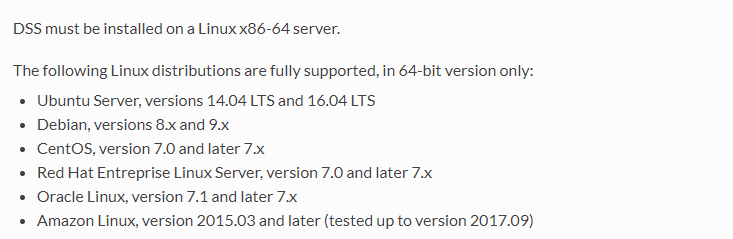
\includegraphics[scale=0.8]{img/software1}
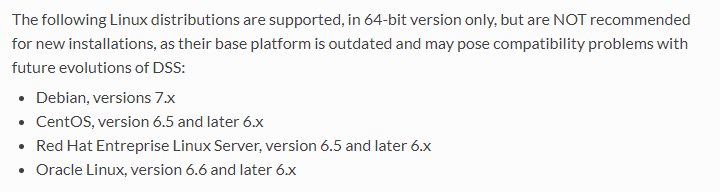
\includegraphics[scale=0.8]{img/software2}

Conclusie

Om Dataiku uit te proberen kan je op de site makkelijk videos en guides vinden die je snel opweg brengen met de tool. Om de tool te gebruiken heb je wel een Linux of Mac OS nodig. Aangezien ik Windows heb moet ik dus voor een review te maken eerst een virtual machine hebben. Als ik uiteindelijk deze tool ga gebruiken voor mijn eigen proof of concept. Dit heeft gelukkig een gratis versie die je altijd kan gebruiken maar deze heeft niet zo veel mogelijkheden als de betalende versie.

\subsection{IBM Watson Analytics}
Je hebt vragen, en je weet zeker dat de antwoorden te vinden zijn in jouw data. Dus wil je een eigen analyse doen. Maar je weet niet zo goed hoe je er aan moet beginnen. Je bent geen Data scientist. Maar je bent wel nieuwsgierig. Omdat je de middelen niet hebt, wacht je meestal op de analyses die je noèdig hebt van IT en dat kan weken duren. Stel je nu eens voor dat jij zelf analyses kan toepassen op jouw data. Hierin komt IBM Watson Analytics tot de redding. Dit is een smart data discovery solution in de cloud. Dat u begeleidt door het maken van analyses. Het automatiseert Data preparation, predictive modeling, en data visualization zodat je jouw nodige data snel hebt. Wachten op IT is dus niet meer nodig. Je moet geen Data Scientist zijn of een training volgen om met deze tool te werken.  

Op de IBM Watson Analytics site staat dat Watson Analytics een data-analyse en visualisatieservice is die je kan gebruiken om snel patronen en betekenis in uw gegevens te ontdekken, helemaal alleen. Met guided data discovery, automated predictive analytics en cognitive capabilities, kunt u bij manier van spreken een gesprek hebben met uw gegevens, en krijg je antwoorden die je makkelijk kan verstaan. Of je nu snel een trend moet zoeken, of een team hebt dat gevisualiseerde data moet krijgen in een dashboard. Het is allemaal mogelijk met Watson Analytics.  [Watson]

Software requirements\newline
Het enigste wat je hiervoor nodig hebt is een browser, de volgende browsers worden gesupport.\newline
-Apple Safari 9+
-Google Chrome 51+
-Microsoft Internet Explorer 11
- Mozilla Firefox 47+ and ESR 45+

Conclusie
Watson Analytics maakt gebruik van hun eigen REST API zodat je jouw eigen applicatie makkelijk kan integreren. Ook hier hebben ze op hun site een heleboel videos en guides die je kan terugvinden om snel op weg te geraken met deze tool. Voor dit te gebruiken moet je wel een \$30 betalen. Er is ook een gratis versie maar deze is maar een 14 dagen geldig. 

\subsection{Databricks}
Op hun site laten ze duidelijk zien welke problemen hun product kan oplossen. Ze laten in een video zien hoe A.I. en Big Data steeds meer en meer gebruikt wordt in bedrijven voor hun meer tijd te geven aan hun eigen inovatieve ideeën. Zoals het gebruik van geautomatiseerde image recognition, real time fraud detection of zelfs genome sequencing. Dit zorgt ervoor dat bedrijven anders gaan werken. Vervolgens laten ze een data engineer aan het woord. Data engineers transformeren en kuisen data op, Data scientists maken en testen machine learning models. Maar het is niet makkelijk om de Data engineers en scientists hun werk te vertalen naar business uitkomsten. Iedereen heeft verschillende vaardigheden. De een gebruikt Python, de ander Scala. Dit maakt het samenwerken moeilijker. Ze spenderen 90\% van hun tijd aan het maken van complexe data pipelines en dergelijke voor nog enkel maar de data klaar te stomen voor dit dan te analyseren. Hierdoor wordt beveiliging maar een na gedachte en innovatie een verre droom. Hiervoor is Databricks dan de ideale oplossing. Met hun unified data management zijn er dan geen problemen meer met data scientists en engineers hun verschillende vaardigheden. Ze maken gebruik van frameworks zoals TenserFlow. Hun clusters zitten in een cloud. Het is van de makers van Apache spark en is zo een 100 keer sneller dan hun open source stuk. Waardoor het team bijna direct data kan beschikbaar maken voor hun analisten. 

De software requirements kon ik niet vinden voor Databricks.

\section{Welke frameworks, visuele tools en scripting tools heb ik nodig om zelf zo een oplossing te bouwen?}
\label{ch:Onderzoeksvraag2}
Hoe maakt men nu zelf zo een oplossing? Dat is hier een van de vragen. Hoe begint men hieraan? We kunnen niet zomaar even op het web googelen, “How to make your own big data analyzer” of iets in die zin. Uiteindelijk bestaan er al een tal van frameworks en tools die hiervoor gebruikt kunnen worden. Zelfs tools die je misschien al kent maar waar je niet direct aan dacht. Zoals Excel. Maar waarom zouden we zelf tools nodig hebben ?

\subsubsection{Waarom tools gebruiken?}
Door het gebruik van tools kan men sneller en makkelijker werken.
Men kan sneller werken vanwege reeds geautomatiseerde stappen in het machine learning proces. Het alternatief is dat men alles van bij het begin moet maken .Wat veel langer kan duren dan gewoon een tool te gebruiken die men vindt op het web.
Het is makkelijker omdat er geen tijd nodig is voor zelf aan research te doen over hoe men bepaalde technieken moet gaan implementeren. Men kan in plaats van hieraan kostbare tijd te spenderen zoeken naar de juiste tool die jij nodig acht. Het alternatief is dat men een expert moet zijn in elke stap van het proces om het te kunnen implementeren. Wat veel onderzoek, oefenen vergt om de technieken te begrijpen.

\subsubsection{Platforms versus Libraries}
Er zijn veel Machine Learning tools, meer als genoeg waardoor je je al snel overwelmt voelt. Daarom is het nog geen slecht idee om Machine Learning tools te gaan onderverdelen in “Platforms” en “Libraries”. Een platform biedt alles wat je nodig hebt om een project te laten draaien. Terwijl een library enkele delen van wat je nodig hebt voor een project te starten aanbiedt. Dit is geen perfecte onderscheiding, aangezien sommige platforms soms libraries zijn en sommige libraries een grafische user interface geven. Voor ons kan dit toch wel een goede scheidingslijn vormen.

\textbf{1. Machine Learning Platform} \newline
Een Machine Learning platform biedt mogelijkheden om een ML project van begin tot eind te voltooien. Namelijk, sommige data-analyse, data-voorbereiding,modellering en algoritme evaluatie en selectie
Kenmerken van machine learning platforms zijn:\newline
-Ze bieden mogelijkheden die in elke stap nodig zijn in een machine learning project.\newline
-De interface mag grafisch zijn, command line of een combinatie van beiden.\newline
-Ze bieden een losse koppeling van functies waardoor u de stukken aan elkaar moet knopen voor uw specifiek project \newline
-Ze zijn op maat gemaakt voor algemeen gebruik in plaats van snelheid, schaalbaarheid of nauwkeurigheid.\newline

Voorbeelden van Machine Learning platforms\newline
-WEKA Machine learning workbench\newline
-R Platform\newline
-Pandas \newline

\textbf{2. Machine Learning Library} \newline
Een machine learning library biedt mogelijkheden voor het voltooien van een deel van een Machine Learning project. Een library kan bijvoorbeeld een verzameling modelleringsalgoritmen bieden
Kenmerken van machine learning libraries zijn:\newline
-Ze bieden een specifieke mogelijkheid voor een of meer stappen in een Machine Learning project.\newline
-De Interface is meestal een API(Een verzameling definities op basis waarvan een computerprogramma kan communiceren met een ander programma of onderdeel)\newline
-Ze zijn afgestemd op een specifiek gebruik, probleemtype of omgeving.\newline
Voorbeelden van machine learning libraries zijn:\newline
-Scikit-learn (Python)\newline
-JSAT (Java)\newline
-Accord Framework (.NET)

\subsection{Machine Learning Tool interfaces}
Een andere handige manier om na te denken over machine learning tools is door de interface die ze bieden. Dit kan verwarrend zijn, omdat sommige tools meerdere interfaces bieden. Niettemin biedt het een startpunt en misschien een punt van differentiatie om u te helpen bij het kiezen van een machine learning tool.
Hieronder zijn enkele voorbeelden van veelgebruikte interfaces.\newline
\textbf{1.Graphical User Interface (GUI)}\newline
Machine learning tools bieden een Graphical User Interface , ”point and click” en een focus op visualisatie. 
De voordelen van een grafische gebruikersinterface zijn:\newline
- Stelt minder technische gebruikers in staat om aan ML te doen.\newline
- Focus op het proces en hoe je het meeste uit ML technieken kan halen.\newline
- De gebruiker krijgt een meer gestructureerd beeld voor zich.

Enkele voorbeelden van ML tools met een grafische interface zijn:\newline
-KNIME \newline
-RapidMiner \newline
-Orange \newline

\textbf{2. Command Line Interface} \newline
ML tools bieden een command line interface met command line programma’s, command line parameterisatie met een focus op input en output. De voordelen van command line user interface zijn: \newline
-Hiermee kunnen mensen die goed overweg kunnen met de command line ook makkelijk door hun ML projecten. \newline
-Biedt veel kleine gerichte programma’s of programma modes voor specifieke subtaken van een ML project. \newline
-Stelt machine learning taken af op basis van de vereiste input en output die moet worden gegenereerd.\newline
Een paar voorbeelden van ML tools voor een command line interface zijn:\newline
-Waffles\newline
-Weka Machine Learning Workbench

\textbf{3. Application Programming Interface(API})\newline
Machine learning tools kunnen u ook een API aanbieden waarmee u zelf kunt bepalen welke elementen u moet gebruiken en hoe u ze precies kunt gebruiken binnen uw eigen programma’s. De voordelen voor API zijn:\newline
-Je kan machine learning integreren in eigen software projecten.\newline
-Hiermee kan je jouw eigen machine learning tools maken.\newline
-Biedt flexibiliteit om eigen processen en automatiseringen te gebruiken voor machine learning projecten.\newline
-Laat toe om uw eigen methoden te combineren met die van de libraries.\newline
Voorbeelden van machine learning tools met API\newline
-Pylearn2 (python)\newline
-Deeplearing4j (java)\newline
-LIBSVM (C)\newline
-TenserFlow(Java, Go, C)\newline

\subsection{Local versus Remote Machine Learning Tools}
Een laatste manier om machine learning tools te vergelijken is door na te gaan of de tool local of remote is
Een local tool is een tool die u lokaal kunt downloaden, installeren en gebruiken, waarbij als externe tool op een externe server wordt uitgevoerd. Dit onderscheid kan ook een beetje troebel zijn omdat sommige tools op een lokale of externe manier kunnen worden uitgevoerd. En uiteindelijk kunt u bijna elk tool als een gehoste oplossing op uw eigen servers configureren. Toch kan dit nog een nuttig onderscheid zijn.

\textbf{1. Local Tools} \newline
Een lokale tool wordt dus zoals de naam zegt, lokaal gedraaid. \newline
- Het wordt op maat gemaakt voor gegevens en algoritmen in het geheugen. \newline
- Je hebt controle over runconfiguratie parameterization. \newline
- U kan het integreren in uw eigen systeem om aan uw behoeften te voldoen. \newline

Voorbeelden van lokale tools zijn:  \newline
Shogun Library (C++) \newline
GoLearn (Go) \newline

\textbf{2. Remote Tools} \newline
Een remote tool wordt gehost op een server en wordt opgeroepen vanuit een lokale omgeving. Deze tools worden vaak Machine Learning as a Service (MLaaS) genoemd. \newline
- Speciaal gemaakt voor uitbereiding, kan worden uitgevoerd op grotere datasets. \newline
- Werkt op meerdere systemen, meerdere kernen en shared memory. \newline
- Minder algoritmen vanwege de aanpassingen die nodig zijn om op schaal te werken. \newline
- Eenvoudigere interfaces , waardoor er minder controle is over run configuratie en parameter aanpassingen van algoritmen. \newline
- Geïntegreerd in uw lokale omgeving via remote procedure calls. \newline
Voorbeelden van remote tools: \newline
- Google Prediction API \newline
- AWS Machine Learning \newline
- Microsoft Azure Machine Learning.


\subsection{Samenvatting}
In dit deel hebben we ontdekt waarom tools dus zo belangrijk zijn als men aan machine learning wil doen. Zonder al deze handige ML tools zouden we al deze technieken zelf moeten maken en implementeren, wat een zeer goede expertise vereist. In dit stuk heeft men ook aangetoond dat er verschillende soorten ML tools zijn die men kan onderscheiden.\newline
-Platforms versus Libraries \newline
- Graphical User Interfaces versus Command-Line Interface Versus Application Programming Interfaces \newline
- Local versus Remote 

\subsection{Conclusie}
Zoals men kan zien zijn er zeer veel tools waaruit men kan kiezen. Met elk hun sterktes en zwaktes, elke tool dat werd opgenoemd heeft men niet apart uitgelegd vanwege het aantal. Hieruit kunnen we dus goed beslissen welke soort tool we nodig zullen hebben. En vervolgens daaruit dan selecteren welke tool we uiteindelijk gaan gebruiken.\newline\newline
\textbf{Platform of libraries?}\newline
een platform is een kant en klare tool eigenlijk wat niet veel ruimte laat voor eigen modificaties. Wat ons kan belemmeren. Bij deze kiest men voor  libraries\newline
\textbf{GUI, Command Line of API?}\newline
Alhoewel het gebruik van GUI tools makkelijker is voor beginners, gaat men toch kiezen voor API. Kiest men toch voor API. De API laat toe om zelf een machine learning tool te maken. En dat is uiteindelijk wat men wou bereiken in deze bachelorproef.
\textbf{Local of remote ?} \newline
Dit maakt niet veel uit voor deze bachelorproef. Men gaat hier gaan voor hetgeen wat men het eenvoudigste vindt. Local.

De tool definitie die we hebben gekozen is : Library , API, Local
Na wat zoeken op het web heeft men al snel een paar tools gevonden die aan onze definitie voldoet.

\subsection{Tenserflow}
Algemene informatie over tenserflow

\subsection{Deeplearning4j} 
Algemene informatie over Deeplearning4j

\subsection{Conclusie}
vergelijken

\section{Welke Dataset gaan we gebruiken en hoe verkrijg ik deze data?}
De manier waarop men deze vraag moet interpreteren is eigenlijk welke parameters/variabelen hebben we zeker nodig in een data set om churn te kunnen voorspellen? Eerst en vooral moet men besluiten of er gaat gewerkt worden met supervised of unsupervised learning. In de literatuur studie heeft men hierover reeds het verschil uitgelegd. \newline
Supervised Machine Learning is wanneer we input variabelen en output variabelen hebben. Het doel is dat men de functie zo willen uitvoeren dat we met een nieuwe input waarde de output waarde kunnen voorspellen\newline
Unsupervised Machine Learning is wanneer men enkel input waarden heeft zonder de output waarden. Het doel hiervan is dat men meer over de input data te weten komt.\newline
Aangezien we niet onmiddellijk meer informatie willen over de input waarden maar wel willen voorspellen welke de output zal zijn, namelijk of een klant gaat churnen ,ja of neen ,1 of 0. Zou men graag een data set willen waar het resultaat ook aanwezig is in de data set.\newline
Dus men kan al één conclusie trekken. De dataset moet een label hebben. In de vorm van Churn ja of neen.\newline
Voor aan gesuperviseerd leren te doen moet men niet enkel output hebben. Daarmee zijn we niet veel. Er moet ook nog input aanwezig zijn. Deze input is eigenlijk alle data wat we weten over deze ene klant. Elke bedrijf segmenteert zijn klanten. In de literatuur studie ziet men hoe men klanten moet gaan onderverdelen. Dankzij model gebaseerde segmentatie kan men makkelijk heel veel variabelen als input meegeven. Betalingsmethoden, tijd, locatie, prijs, hoeveelheid gekocht, korting, het weer, enz…

\subsection{Telco-Customer-data set}
Deze dataset bevat info die ons kan helpen om het gedrag van klanten te gaan voorspellen. Deze data set heeft men gevonden op de IBM Watson Analytics site in een tutorial. In de tutorial gaat het als volgt. Een telecom bedrijf is bezorgd over het aantal klanten dat ze verliezen aan hun concurrentie. Ze willen te weten komen wie er gaat vertrekken. In het voorbeeld op de site moet je u inbeelden dat jij de analist bent in hun bedrijf en dat jij dit moet uitzoeken.

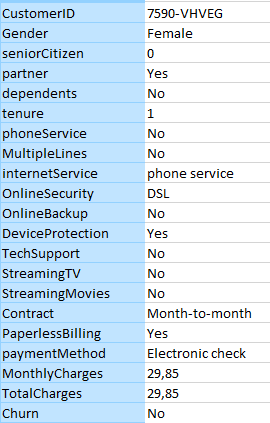
\includegraphics[scale=0.8]{img/dataset}

De data set heeft informatie over

•	De klanten die het bedrijf zijn verlaten. De laatste kolom Churn. \newline
•	Services waar elke klant voor geabonneerd is, phones,multiple lines, internet,online security,online backup,device,protection,tech support, 		 streaming TV en movies. \newline
•	-Profiel informatie van de klant, hoelang ze al klant zijn,contract,payment method,paperless billing, monthly charges, en total charges\newline
•	-Demographic info over de klanten gender, age, range en of ze partners en dependents hebben.

Hier ziet men eigenlijk al goed dat deze data set een tal van onze gewenste variabelen bevat.
Maar we moeten onze dataset nog opschonen. Dit komt voor in de proof of concept.

\section{Welk Model dien ik hiervoor op te zetten?}

\section{Kies ik beter scripting tools zoals python?}











